%---------------------------------------------------------------
\chapter{Ray tracing and acceleration data structures}
\label{chap:theory}
%---------------------------------------------------------------

\begin{chapterabstract}
 
This chapter focuses on exploring ray tracing and acceleration data structures used for ray tracing. In particular it will delve into bounding volume hierarchies, starting from the theoretical foundations of cost functions, construction methods and traversal all the way to specific research papers focused on enhancing and expanding the existing techniques. The main goal of this chapter is to enrich the reader and welcome him into the topic of bounding volume hierarchies. Special focus will be given to GPU friendly algorithms and techniques.

\end{chapterabstract}

\begin{figure}[h!tb]
    \centering
    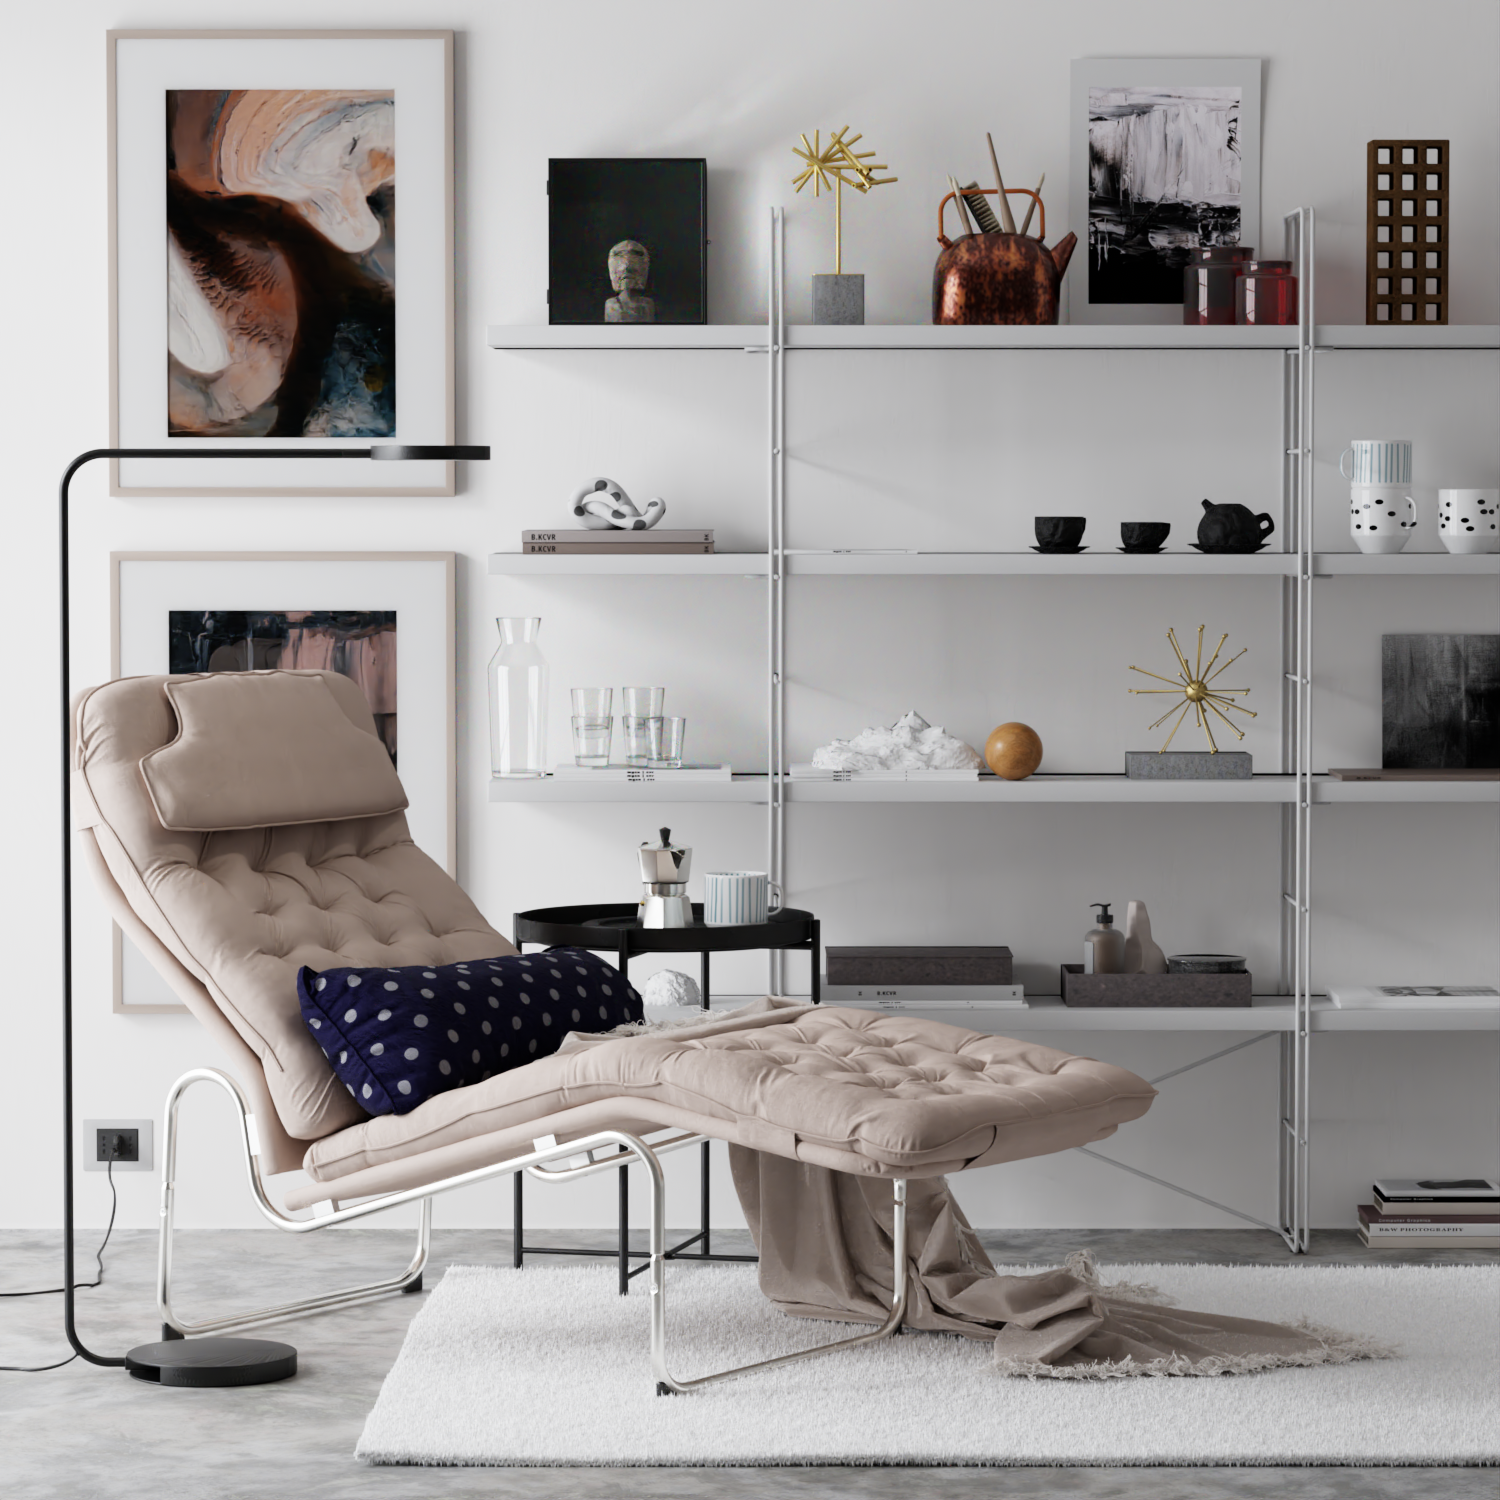
\includegraphics[width=0.95\textwidth]{images/pbr renders/fancy_render_pbr2.png}
    \caption{Rendering capabilities of ray tracing. Courtesy of the PBR book \cite{pbr4}}
    \label{fig:pbr4_render}
\end{figure}

\section{Ray tracing}

Ray tracing is a physically based rendering technique used to render images by simulating the propagation of light in a scene made up of primitives (typically triangles). The fundamental idea is to trace rays from the camera through each pixel into the scene, finding their interactions with geometry and materials. Compared to traditional rasterization methods, ray tracing naturally supports effects such as reflections, refractions, and shadows, making it particularly suitable for realistic image synthesis. Figure \ref{fig:pbr4_render} shows the capabilities of this rendering technique.

A basic approach to ray tracing was introduced by Whitted~\cite{W80}, who proposed a recursive algorithm for handling reflection and refraction. In this model, primary rays are cast from the camera into the scene to determine visible surfaces. At each intersection point, additional rays are generated to simulate reflected and refracted light, as well as shadow rays to determine the visibility of light sources (if the intersection point receives energy from them). This recursive process enables the simulation of complex optical effects, although it is limited in its ability to model diffuse global illumination.~\cite{W80}

A more general formulation of light transport is given by the rendering equation, introduced by Kajiya~\cite{K86}. The rendering equation expresses the outgoing radiance at a point as the sum of emitted and reflected radiance over all incoming directions. It is defined as~\cite{K86}:
\begin{equation}
L_o(x, \omega_o) = L_e(x, \omega_o) + \int_{\Omega} f_r(x, \omega_i, \omega_o) \, L_i(x, \omega_i) \, (\omega_i \cdot n) \, d\omega_i,
\end{equation}
where $L_o$ is the outgoing radiance, $L_e$ is the emitted radiance, $f_r$ is the bidirectional reflectance distribution function (BRDF), and $L_i$ is the incoming radiance. The integral is taken over the hemisphere $\Omega$ above the surface point. This equation provides a physically accurate description of light transport but does not have a closed-form solution in the general case, requiring numerical approximation methods such as Monte Carlo integration.~\cite{K86}

The high computational complexity of ray tracing stems from the need to evaluate ray-scene intersections for a large number of rays. For a scene consisting of $N$ geometric primitives, a naive ray tracing approach requires testing each ray against all primitives, resulting in $O(N)$ intersection tests per ray. Since realistic rendering requires tracing millions to billions of rays, the overall complexity becomes unbearable. Furthermore, recursive ray generation (e.g., for reflections and global illumination) increases the number of rays exponentially with recursion depth.

To address this issue, acceleration data structures (ADS), such as bounding volume hierarchies (BVH), are employed to reduce the number of intersection tests. These structures divide the scene geometry in a hierarchical manner (either by dividing space or objects), allowing large groups of primitives to be culled with a single intersection test. As a result, the expected complexity of ray traversal can be reduced to approximately $O(\log N)$ for well-constructed hierarchies, making ray tracing feasable for complex scenes.

The challenges of ray tracing are further amplified on modern parallel architectures such as GPUs. The irregular memory access patterns, control flow divergence, and varying workloads per ray complicate efficient parallel implementation. In particular, traversal of hierarchical data structures such as BVHs introduces branch divergence and incoherent memory access, which can significantly degrade performance. These challenges motivate the development of specialized data structures and algorithms optimized for GPU execution, which are the focus of this thesis.

% ----------------------------------------
\newpage
\clearpage
\section{Acceleration data structures}
% - Základní typy datových struktur používaných pro ray tracing

\begin{figure}[h!tb]
    \centering
    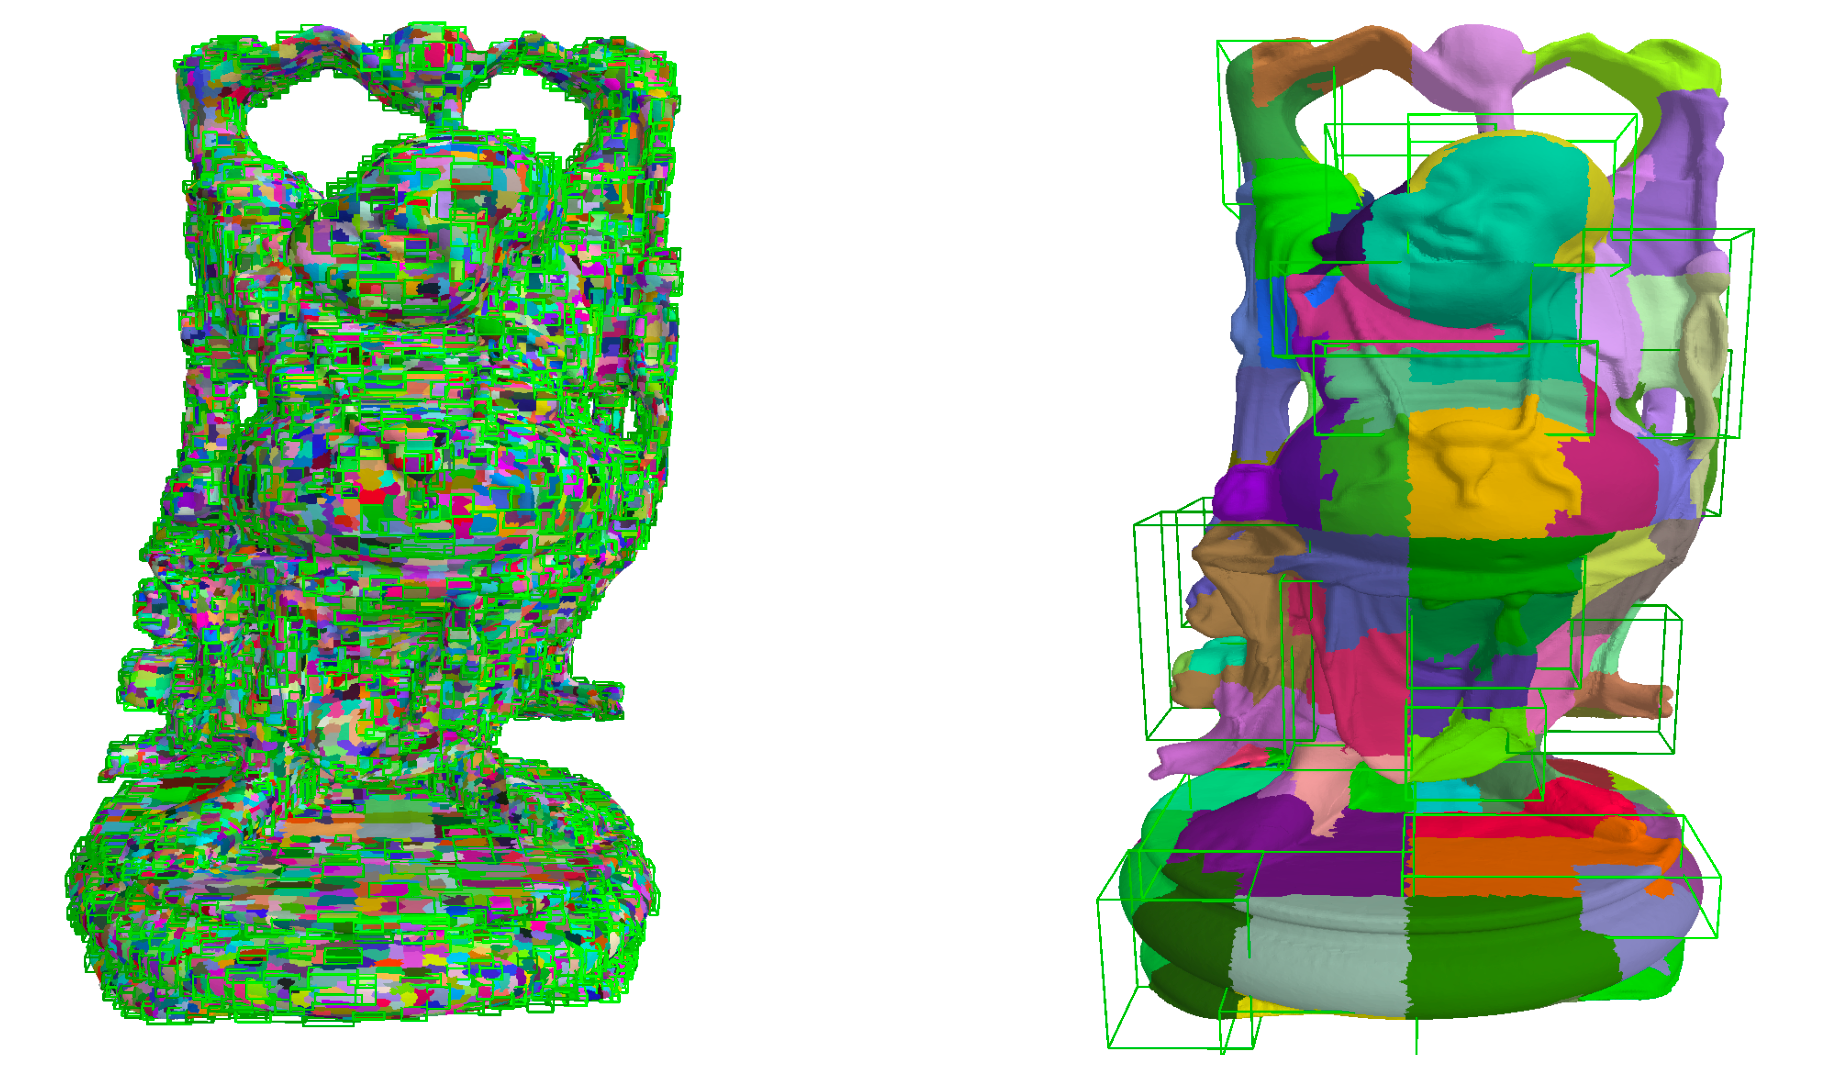
\includegraphics[width=0.95\textwidth]{images/BVH_visualisation_PLOC.png}
    \caption{Visualization of the different stages of BVH construction. \cite{MB17}}
    \label{fig:ploc_clusterint_example}
\end{figure}

The problem of realistic image synthesis using ray tracing is the sheer number of rays needed that must be traced to get plausible results. Otherwise, the resulting images are plagued with high-frequency noise. The light transport simulation is based on a basic geometric operation, \textit{finding the nearest intersection} of a given ray with the scene. We might also want to find \textit{any intersection} or \textit{all intersections} with the scene. The query into the scene is usually described as a \textit{ray} with an \textit{origin} and a \textit{direction}. Without any optimizations, we would have to compute the ray-scene intersections one by one for each ray-primitive pair. This becomes computationally unfeasible very quickly as scenes might consist of millions of primitives, and the number of rays is at least as large as the number of pixels in the desired image. \cite{Meister2021}

The simulation of light transport can be accelerated, for example, by sorting scene primitives into efficient spatial data structures, namely acceleration data structures. In the last decades, the most popular acceleration data structure for ray tracing is the bounding volume hierarchy \cite{Cla76}. For that reason, this section will focus on it in favor of other ADS.

This thesis will focus on the bounding volume hierarchy data structures that are used for ray tracing. There are many other data structures used for ray tracing, but over the years BVH has become the de facto industry standard when it comes to ray tracing acceleration. 

Other data structures include, for example, Octrees that were first introduced in 1982 \cite{M82} and first used for ray tracing in 1984 \cite{G84} and KD-trees that were first introduced in 1975 \cite{B75} and first used for ray tracing in 1990 \cite{MB90} using the surface area heuristic \cite{GS87} (more on this later). However, these data structures are not within the scope of this thesis.

\subsection{Bounding volume hierarchy}
A \textit{bounding volume hierarchy} is a rooted tree with a branching factor (denoted \textit{k}). Individual nodes have two types: interior nodes, which hold pointers to child nodes, and leaf nodes, which hold references to scene primitives. All nodes contain a bounding volume that tightly wraps around the geometry in the leaves. BVH was originally a binary tree, but in recent years a higher branching factor has become favorable. In the context of ray tracing, the bounding volume of choice is almost exclusively an \textit{axis aligned bounding box} (AABB). It is used for its small memory footprint and computationally easy intersection with rays. Other bounding volumes are sometimes used for specific cases. For example, \textit{bounding spheres}, \textit{oriented bounding boxes} (OBB), or, more recently, more experimental \textit{skewed oriented bounding boxes} (SOBB) — more on them in a later Section \ref{sec:sobb} — are being used. BVH can theoretically be used with an arbitrary number of dimensions, but in rendering, where scene primitives are 3D entities, more than 3 dimensions are rarely needed.

The popularity of BVHs comes from the following advantages:

\paragraph{Predictable memory footprint} The number of primitives directly influences the memory footprint. Scene primitives are usually referenced only once. In that case, the BVH is made up of at most $2n-1$ nodes (where $n$ is the number of primitives). This corresponds to a binary BVH with a single primitive in each leaf. If the branching factor \textit{k} is higher, the number of internal nodes decreases. The same applies, but for leaf nodes, when more than one primitive is stored in a single leaf node. \cite{Meister2021}

\paragraph{Robust and efficient query} Due to the hierarchical structure and the use of objects instead of spatial splitting, the BVH is robust to any scene distribution. For example, the \textit{"teapot in the stadium problem"}\footnote{ is a very small and detailed object inside a large object — a vast difference in scale can lead to poor splitting.}. Using spatial splitting data structures, we would not cull the space efficiently enough, but using BVH, we are able to efficiently prune branches when traversing the tree and quickly get rid of the branches that do not intersect a given ray. BVH traversal algorithms typically have a small and compact traversal state and can be efficiently parallelized \cite{Meister2021}. This results in great ray tracing performance, in most cases at least as good as KD-trees \cite{VHB16}, taking their place as the best data structure for ray tracing \cite{Hav00}.

\paragraph{Scalable construction} Various construction algorithms for BVH exist, ranging from very fast to complex algorithms, providing high quality results in exchange for longer build times. With this flexibility, we can tailor the balance to our needs between construction speed and BVH quality. The most straightforward metric for BVH quality in the field of ray tracing is the speed in millions of rays cast per second (MRays/s). We usually optimize the total time to render the image, which is the sum of the ray casting and the constuction time. In real-time applications, we usually have a small budget for both these phases, thus we have to limit ourselves to a medium quality BVH in exchange for faster construction. This works because the number of rays that can be cast is lower and it is not worth investing more time into constructing a higher quality BVH. On the other hand, in offline rendering, where the time budget is not as tight, we can afford to invest more time in construction because the number of rays cast is significantly higher than in real-time rendering, yielding a net performance gain. \cite{Meister2021}

\paragraph{Dynamic geometry} Spatial subdivision suffers from the inability to easily refit bounding volumes (such as the KD-tree). Compared to BVH, where the reffitting can be done by a simple bottom up pass. Also, since fast BVH construction methods are available, it is suitable for use with dynamic geometry through straightforward rebuilding. \cite{Meister2021}

\paragraph{}A basic top down construction of BVH can be done recursively by splitting the set of primitives info subsets. The pseudocode is shown in Algorithm \ref{alg:top-down-bvh}.

\begin{algorithm}[h!tb]
\caption{Basic top-down BVH construction algorithm\cite{Meister2021}.}
\label{alg:top-down-bvh}
\begin{algorithmic}[1]
\While{stack is not empty}
    \State pop \textit{node} from the top of the stack
    \If{termination criteria for \textit{node} are met}
        \State make \textit{node} info leaf
    \Else
        \State split primitives in \textit{node} into \textit{children}
        \State assign \textit{children} as child nodes of \textit{node}
        \For{child in node}
            \State push \textit{child} onto the stack
        \EndFor
    \EndIf
\EndWhile
\end{algorithmic}
\end{algorithm}

\paragraph{} To find the nearest neighbor, the BVH can be traversed in a top down manner, starting from the root. A depth-first-search approach is usually used, storing interior nodes in a stack during traversal and traversing first the nodes that potentially contain the nearest intersection. We store the distance to the nearest intersection found so far and cull the nodes that are further. A basic traversal algorithm is illustrated in Figure \ref{fig:bvh-traversal} and its pseudocode is shown in Algorithm \ref{alg:bvh-traversal}.

\begin{figure}[h!tb]
    \centering
    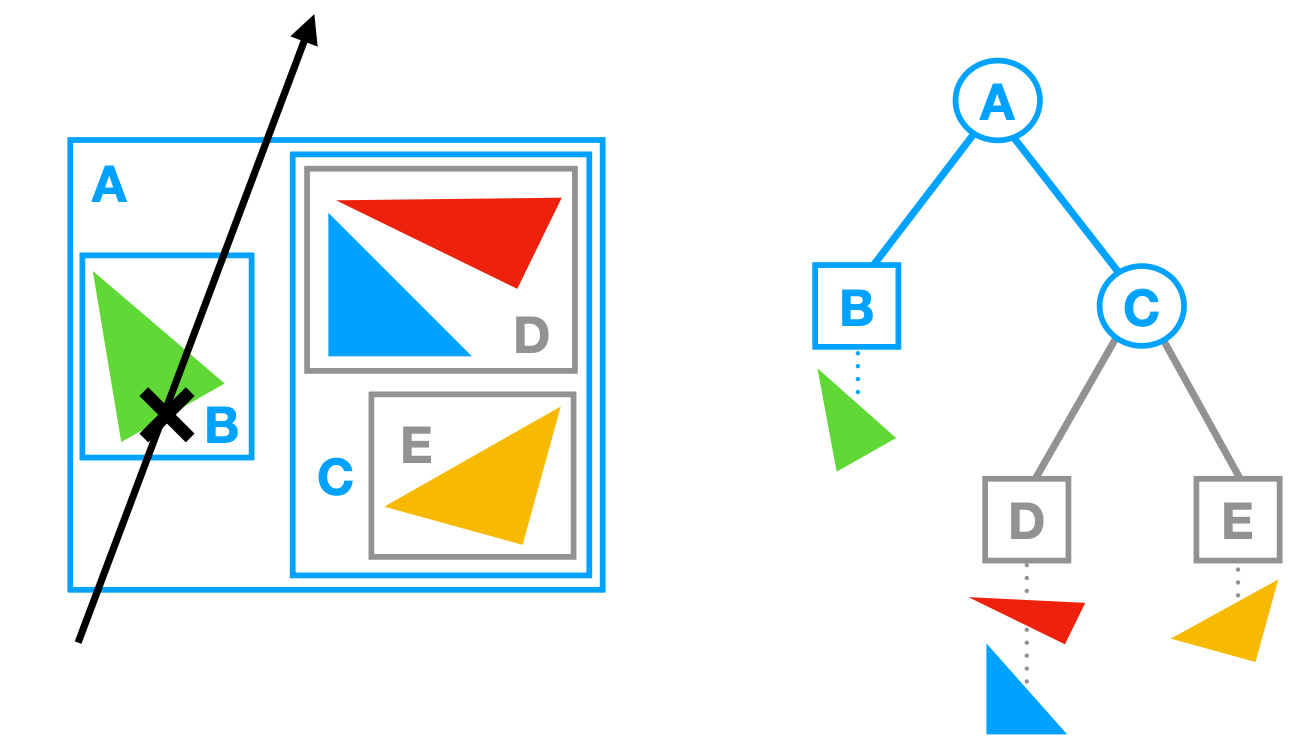
\includegraphics[width=0.9\linewidth]{images/BVHTraversal.png}
    \caption{Example BVH over 4 primitives. Constructed tree includes bounding volumes (AABBs). While traversing the scene we cull the entire subtree of node C since the ray does not intersect its bounding box\cite{Meister2021}.}
    \label{fig:bvh-traversal}
\end{figure}

\begin{algorithm}[h!tb]
\caption{Basic stack-based BVH traversal algorithm\cite{Meister2021}.}
\label{alg:bvh-traversal}
\begin{algorithmic}[1]
\State push \textit{root} onto the stack
\While{stack is not empty}
    \State pop \textit{node} from the top of the stack
    \If{\textit{ray} intersects \textit{node}}
        \If{\textit{node} is not a leaf}
            \For{\textit{child} in \textit{node}}
                \State push \textit{child} onto stack
            \EndFor
        \Else
            \For{\textit{prim} in \textit{node}}
                \State test whether \textit{ray} intersects \textit{prim}
            \EndFor
        \EndIf
    \EndIf
\EndWhile
\end{algorithmic}
\end{algorithm}

\subsubsection{Cost function}
\label{sec:cost-function}

The quality of a BVH can be estimated using a cost function. Cost functions attempt to capture the expected number of operations needed for finding the nearest intersection with a given ray. The cost of a BVH rooted in node $N$ is described by the equation \cite{Meister2021}:
\begin{equation}
    c(N) =
    \begin{cases}
        c_T + \displaystyle\sum_{N_c} P(N_c \mid N) c(N_c) & \text{if } N \text{ is interior node}, \\
        c_I \lvert N \rvert & \text{otherwise},
    \end{cases}
    \label{eq:cost-function}
\end{equation}
where $c(N)$ is the cost of a subtree with root $N$, $N_c$ is a child of $N$, $P(N_c|N)$ is the conditional probability of traversing node $N_c$ when already in node $N$. $|N|$ is then the number of scene primitives in a subtree with root node $N$. The average cost of a traversal step is denoted by $c_T$ and the average cost of a ray-primitive intersection is expressed by $c_I$. The concrete values of these constants are very roughly estimated instead of a precise number of computation steps. In practice, only the ratio of these constants is important, not the absolute values.

\paragraph{Surface area heuristic (SAH) \cite{GS87}} can be used to express conditional probability as geometric probabilities, than means that the ratio of the surface areas of child and parent nodes can be used instead of the conditional probability:
\begin{equation}
    P(N_c \mid N)^{SAH} = \frac{SA(N_c)}{SA(N)},
    \label{eq:sah-conditional-propability}
\end{equation}
where $SA(N)$ denotes the surface area of the bounding volume of node $N$. By substituting Equation \ref{eq:sah-conditional-propability} into Equation \ref{eq:cost-function} and unrolling to remove the recurrence, we get the following:
\begin{equation}
    c(N)^{SAH} = \frac{1}{SA(N)} \left[ c_T \sum_{N_i} SA(N_i) + c_I \sum_{N_l} SA(N_l) |N_l| \right], 
    \label{eq:placeholder_label}
\end{equation}
The problem of finding an optimal BVH is believed to be NP-hard \cite{AK13}.

\paragraph{Other cost functions} exist. The SAH assumes that the rays are uniformly distributed around the scene, with their origins outside. That is unrealistic, and so other cost functions or SAH corrections were suggested. For example, Bittner and Havran \cite{BH09} proposed a method that takes into account the distribution of rays in a scene and then used the ratio of ray hits instead of surface areas, they called it \textit{ray distribution heuristic}. Vinkler et al \cite{VHS12} proposed using the ratio of visible scene primitives, called \textit{occlusion heuristic}. Many more SAH upgrades or completely new methods exist, but that is outside of the scope of this thesis.

\subsubsection{Construction}

In this section, we will summarize the basic construction methods. Basic methods include top-down methods, bottom-up methods, and incremental construction methods. When we already have the BVH tree, it can be transformed or optimized into a wide BVH, for example, by increasing its branching factor by subtree collapsing.

\paragraph{Top-down construction} was adapted from KD-tree construction methods \cite{Wal07}. It starts with the root node that contains the whole scene. In each recursive step, the scene primitives are split into two (or more, based on \textit{k}) disjoint sets that are assigned to the two (or \textit{k}) children of the current node. This continues until the termination conditions are met. The termination conditions usually are the maximum number of primitives in a node/leaf, the maximum depth, or a memory bound. In general, there are exponentially many ways to split scene primitives into disjoint subsets. Even if we perform an optimal split at every step, the final BVH might not be optimal and is very likely to be just a local optimum of the cost function. \cite{Meister2021}

In practice, we split the scene primitives using axis-aligned planes. Each scene primitive is referenced only once, it lives in only one leaf node. We approximate the scene primitive by a single point in space (typically the centroid of the bounding box), of which we can then determine into which disjoint set it belongs. First, we select the best splitting axis either by the spatial median, object median, a cost function, or artificially, such as round-robin or by largest extent. The spatial median splits the bounding box in the middle. The object median selects a splitting point in a way that half of the scene primitives are on each side (this can also be used as a backup splitting method). The cost function split tries to minimize the cost locally, treating the children as leaves.

We can also use the local costs as a termination condition. If the split created has a higher cost than a leaf, we do not split further and create a leaf from the current node.

\paragraph{Bottom-up construction} is an opposite approach to top-down construction by agglomerative clustering \cite{WBKP08}. At first, all scene primitives are clusters of size one. In each iteration, the closest pairs of clusters are merged into larger clusters. The algorithm terminates when there is only one cluster left, the root. The distance of pairs is the surface area of the bounding box that tightly encloses both clusters. In general, agglomerative clustering creates lower cost BVHs, but the construction takes longer. This cost may be deceiving because the optimizations are mostly at the bottom levels of the tree, so, the upper levels might be poorly optimized (unlike in top-down methods). This may lead to worse performance due to the fact that most traversal time is spent in the upper levels. The most expensive part of the method is the nearest neighbor search that has to be done in each iteration for each cluster pair. \cite{Meister2021} 

\paragraph{Incremental construction} works similarly to a heap sort. We start with an empty BVH tree and insert scene primitives one by one. Each primitive is inserted  into an appropriate leaf node that is found by traversing the BVH from the root. If a leaf has too many primitives, it is split into two new leaf nodes and becomes an internal node. This method is useful for streaming and other circumstances where we do not know the full extent of the scene at the beginning of the construction. However, this approach produces lower quality BVHs in general. \cite{Meister2021}

\paragraph{Subtree collapsing} serves to optimize memory overhead, create denser trees, or increase the branching factor of an existing BVH. Bottom-up construction and some other construction or optimization techniques produce BVHs with only one primitive per leaf. Larger leaves might have a better cost (depending on the constants $c_T$ and $c_I$). The collapse of the subtree starts from the leaves up and continues to the root, comparing whether the node cost would be better by merging the child nodes into a larger leaf. If the cost is less than or equal to the current cost, the subtree collapses into a larger leaf. \cite{Meister2021}

\paragraph{Wide BVH} is known as a BVH with a higher branching factor $k$, sometimes denoted as BVH$k$ (e.g., BVH4 or BVH8). Wide BVHs can utilize more computing resources by parallelizing using SIMD/SIMT units, thus enabling a more efficient traversal by testing multiple bounding volumes against the given ray at the same time. Along with that, they are also stored more efficiently in memory since they have fewer interior nodes than binary BVHs (depending on the fullness of the tree).

The caveat is that the wide BVHs have to deal with empty slots (unlike binary BVHs) since it is highly unlikely that each interior node has all its children utilized, especially around the leaf levels of the tree.

Two classes of algorithms exist for wide BVH construction. The first class depends on an already constructed BVH, which it converts into a BVH$k$ by culling interior nodes. The second class builds the wide BVH during construction. \cite{Meister2021}

\subsubsection{Traversal}

\begin{figure*}[h!tb]
    \centering
    \begin{subfigure}{.33\textwidth}
        \centering
        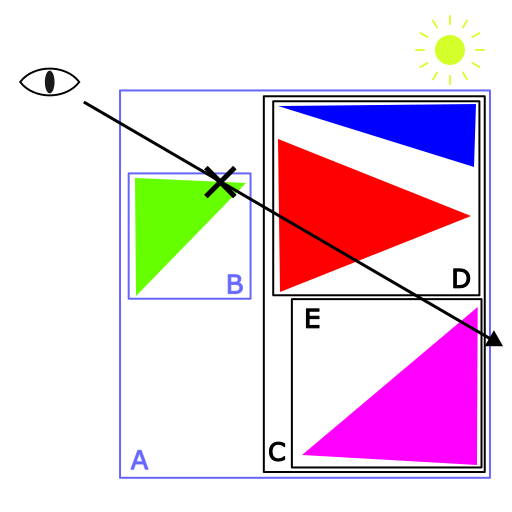
\includegraphics[width=.9\linewidth]{images/FirstHit.png}
        \caption{First-hit traversal.}
        \label{fig:traversal-first-hit}
    \end{subfigure}%
    \begin{subfigure}{.33\textwidth}
        \centering
        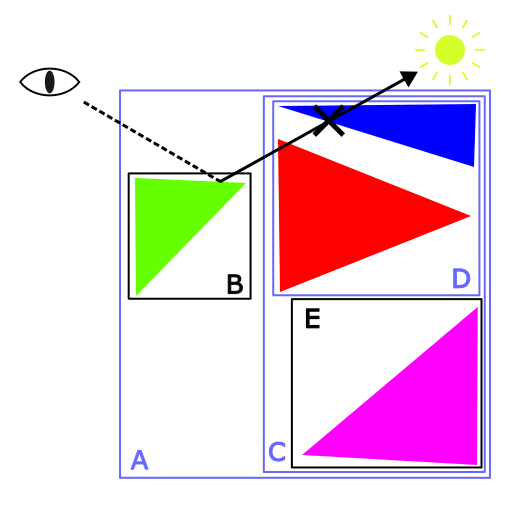
\includegraphics[width=.9\linewidth]{images/AnyHit.png}
        \caption{Any-hit traversal.}
        \label{fig:traversal-any-hit}
    \end{subfigure}%
    \begin{subfigure}{.33\textwidth}
        \centering
        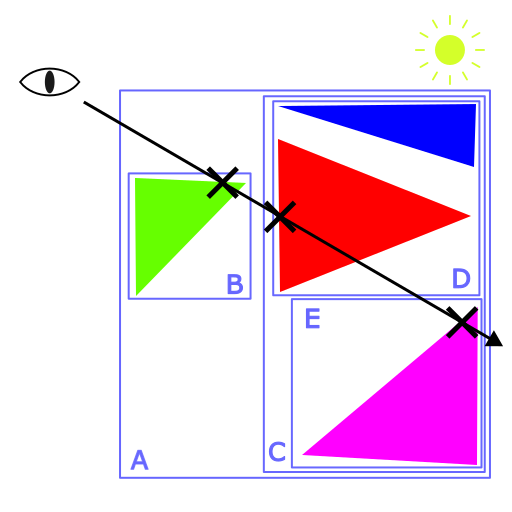
\includegraphics[width=.9\linewidth]{images/MultiHit.png}
        \caption{Multi-hit traversal.}
        \label{fig:traversal-multi-hit}
    \end{subfigure}
    \label{fig:traversal-hit-types}
    \caption{Hit traversal types demonstrated on a simple scene with triangles as primitives, bounding volumes, a camera, and a light source.}
\end{figure*}

The whole point of spatial acceleration data structures for ray tracing is to reduce the number of ray-primitive intersections at the cost of traversing the data structure. In this section the thesis describes the basic types of traversal.

\newpage
\paragraph{}There are three main types of traversal:
\begin{itemize}
    \item First-hit traversal (closest hit); finds the object nearest to the ray origin in the ray direction. The typical use case are primary and secondary rays in ray/path tracing. Figure \ref{fig:traversal-first-hit} shows this hit type.
    \item Any-hit traversal (occlusion test); finds any object in the ray direction starting from the ray origin. This is useful for shadow computation or ambient occlusion. Figure \ref{fig:traversal-any-hit} shows this hit type.
    \item Multi-hit traversal; finds all or \textit{h} closest intersections from the viewpoint. Used when dealing with non-refractive transparent surfaces, it avoids the need to retrace another ray from the root each time a ray hits an object. Figure \ref{fig:traversal-multi-hit} shows this hit type.
\end{itemize}

\paragraph{First-hit traversal} is most used for computing radiance at a shading point and most ray tracing engines are optimized for this kind of traversal. For binary BVHs it is straightforward to efficiently implement this just by pushing the farther child onto the stack and traversing the closer one first. When it comes to wide BVHs, there are $k!$ orders of traversal for branching factor $k$, and each ray may intersect any number of child nodes. Due to this, the child nodes must be ordered from front to back to be efficient. There are two common heuristics for sorting. One option is to simply use the sign of the ray direction and the split axes used during construction. The other option is to use the ray distance to the bounding volumes of the child nodes and sort according to it. When traversing wide BVHs, generally only 0 to 3 child nodes are intersecting, for any $k$, so it is possible to code a preset path to sort this small number of nodes and perform a complete sort only if there are 4 or more intersecting child nodes. \cite{Meister2021}

\paragraph{Any-hit traversal} or occlusion rays account for a large portion of the total rays used for ray tracing, for example when computing soft shadows from area lights, illumination from many lights or evaluating ambient occlusion. There is no need to visit all intersections front to back when calculating occlusion in a scene without any transparent geometry. Traversal can terminate the moment a ray intersects with any object. Any-hit traversal can have its own dedicated BVH with different metrics than first-hit traversal. \cite{Meister2021}

\paragraph{Multi-hit traversal} finds all intersections or $h$ nearest intersections inside a scene along a given ray. It is a generalization of first-hit traversal. Multi-hit traversal addresses the issues that first-hit traversal has with planar objects — self-intersection, particularly when handling two transparent materials next to each other (such as glass and water). Another use case is with reflected and refracted rays. When these rays are traced with a negative $\epsilon$-offset or a positive $\epsilon$-offset, the correct primitive intersections might be repeated or missed completely. There are two types of multi-hit traversal: those that find a limited number of intersections, where we can use a pre-allocated buffer to store the required intersections, and those that need to find all of them. When all intersections are required, it is usually not possible to predict their number. In this case, a method that works without dynamically allocating the list/buffer is preferred due to the overhead of reallocation. The same applies when a lot of intersections are needed. \cite{Meister2021}

\subsubsection{GPU traversal}

Traversal on GPUs is challenging because GPUs execute 32 threads in a parallel SIMD block called a \textit{warp}. This causes issues with non-locality of data access and control flow when using any acceleration data structure. To decrease the wait time of threads in a warp that have already completely traversed the given rays, new rays are loaded from a global work queue using \textit{persistent threads}. The traversal loop can be broken up into two independent loops to mitigate the control flow divergence.  The two loops are: iterating over the hierarchy and iterating over the primitives\cite{AL09}. To distribute the threads between these two loops, each on is implemented as either an \textit{if} block or a \textit{while} block. The So called \textit{if-if} traversal alternates the testing of nodes and primitives if \textbf{any} of those threads need to process an inner or a leaf node, respectively. On the other side in the \textit{while-while} traversal the hierarchy is traversed until all threads reach a leaf node, before all thread switch to iterating over primitives, This might lead to only a single thread being active in a warp, the switch to the other block is conditioned by a waiting thread count threshold instead of waiting for all of them. In addition, to increase the memory throughput at the cost of a few more traversed inner nodes, the traversal is continued, in the case of \textit{while-while} traversal, until a second leaf node is reached. The \textit{persistent speculative while-while} algorithm, which you can find in Algorithm \ref{alg:while-while}, shows the traversal algorithm with all discussed optimizations. \cite{Meister2021}

\definecolor{darkgreen}{RGB}{0,150,0}

\begin{algorithm}[h!tb]
\caption{Persistent speculative while-while traversal algorithm. Speculative traversal of inner nodes is marked in blue and ray fetching for persistent threads in green.\cite{Meister2021}}
\label{alg:while-while}
\begin{algorithmic}[1]
\State \textit{ray} = fetch\_ray()
\State \textit{node} = \textit{root}
{\color{blue}\State \textit{leaf} = $\varnothing$}
\While{{\color{darkgreen}\textit{ray} $\neq \varnothing$}}
    \State /* \textsc{Iteration over the hierarchy} */
    \While{\textit{node} does not contain primitives}
        \State traverse to the next \textit{node}
        \color{blue}
        \If{\textit{node} contains primitives \textbf{and} \textit{leaf} = $\varnothing$}
            \State \textit{leaf} = \textit{node}
            \State traverse to the next \textit{node}
        \EndIf
        \If{number of (\textit{leaf} $ \neq \varnothing$) per warp $>$ \textit{threshold}}
            \State break
        \EndIf
        \color{black}
    \EndWhile
    \State /* \textsc{Iteration over the primitives} */
    \While{\textit{leaf} or \textit{node} contain untested primitives}
        \State perform a ray-primitive intersection test
        \color{darkgreen}
        \If{\textit{ray} is terminated}
            \State \textit{ray} = fetch\_ray()
            \State \textit{node} = \textit{root}
        \color{black}
        \EndIf
    \EndWhile
\EndWhile
\end{algorithmic}
\end{algorithm}

The main performance limiter of GPU traversal is latency \cite{Guthe14} and not memory bandwidth or computation operation speed. There are more optimizations available. For example, loop unrolling can provide more instructions that the GPU is able to reorder, or having a wider BVH can help make individual instructions more independent. Sorting children using a predefined sorting network instead of a full sorting algorithm can also help to have more independent instructions. \cite{Meister2021}


% ----------------------------------------
\clearpage
\section{Parallel locally ordered clustering for BVHs}

The authors \cite{MB17} propose an algorithm using parallel locally-ordered clustering (PLOC) for BVH construction. The algorithm consists of two main ideas: First, locally-ordered clustering on a large number of clusters is performed in parallel. Second, to identify the nearest neighbors for clusters, Morton codes are used to sort and search the sorted sequence with local exploration instead of a complete nearest neighbor search.

Firstly, the thesis will describe these two ideas in more depth in the coming sections, and then it will provide a description of the original authors complete algorithm.

\subsection{Parallel locally ordered clustering}
\label{sec:ploc-aglomerative-clustering}

The starting point of the agglomerative clustering algorithm is a scene with primitives (triangles) forming $n$ clusters with a single primitive per cluster ($n$ being the number of primitives). These starting clusters are the leaves of the BVH. The algorithm then builds the higher levels by merging the clusters from the lower levels.

The distance function $d$ between two clusters $C_1$ and $C_2$ is defined as the surface area $A$ of an AABB that tightly encloses $C_1$ and $C_2$ \cite{WBKP08}:

\begin{equation}
    d(C_1, C_2) = A(\mathcal{B}(C_1 \cup C_2)) = A(\mathcal{B}(\cup(C_1, C_2))),
\end{equation}

where $\cup(C_1, C_2)$ is the clustering operator and $\mathcal{B}(C)$ is the AABB tightly enclosing cluster $C$. The function $d$ conforms to a non-decreasing property:

\begin{equation}
    d(C_1, C_2) \leq d(C_1 \cup C_3, C_2) : \forall C_1, C_2, C_3. 
\end{equation}

Walter et al. \cite{WBKP08} used the non-decreasing property and proposed the \textit{locally-ordered} agglomerative clustering algorithm. No better neighbor will emerge in the future if the nearest neighbors of two clusters \textit{mutually correspond} (both are each others nearest neighbors). The algorithm can then safely merge the mutually corresponding clusters together. This property is exploited in the following algorithm and is applied to all pairs of mutually corresponding clusters in parallel.

\subsection{Approximate nearest neighbor search}

\begin{figure*}[h!tb]
    \centering
    \begin{subfigure}{.5\textwidth}
        \centering
        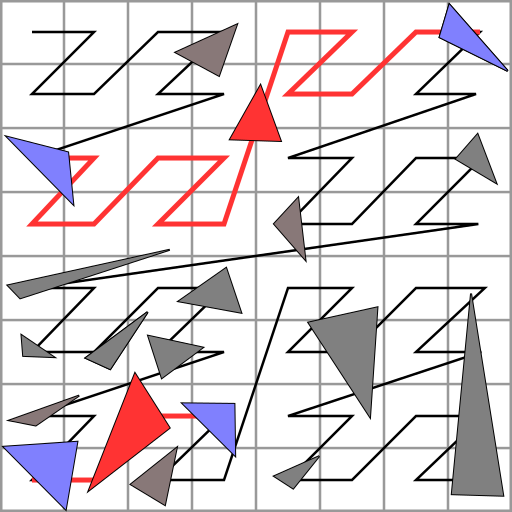
\includegraphics[width=.8\linewidth]{images/PLOC_nnsearch_r1.png}
    \end{subfigure}%
    \begin{subfigure}{.5\textwidth}
        \centering
        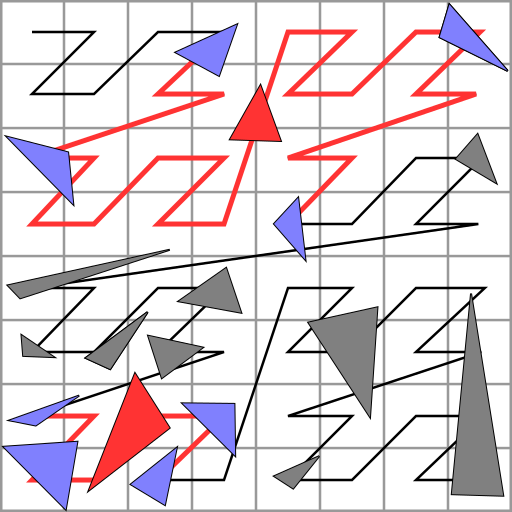
\includegraphics[width=.8\linewidth]{images/PLOC_nnsearch_r2.png}
    \end{subfigure}
    \caption{PLOC nearest neighbor search for $r = 1$ (left) and $r = 2$ (right). Clusters (red) search for their nearest neighbor (blue) along the Morton curve. \cite{MB17}}
    \label{fig:ploc-nn}
\end{figure*}

Each cluster needs to identify its nearest neighbors. Naïve evaluation would take $\mathcal{O}(n^2)$ time for $n$ clusters, which is inefficient and insufficient for large $n$.

The authors propose an alternative way to identify the nearest neighbors for all clusters. The clusters are sorted based on their centroids Morton codes. Then, for each nearest neighbor search, the algorithm just needs to use the 1D range search of the Morton curve to identify the nearest neighbor. To search for the nearest neighbors of cluster $C_i$ with index $i$, it searches the sorted sequence in the interval $\langle i-r,i+r \rangle$, where $r$ is the search radius. For every cluster $C_j, j \in \langle i-r,i+r \rangle \setminus {i}$, the algorithm evaluates the distance between the two clusters $d(C_i,C_j)$. The candidate $C_j$ with the smallest distance $d$ is selected as the nearest neighbor. An illustration can be seen in Figure \ref{fig:ploc-nn}. \cite{MB17}

Even though this method only finds the approximate nearest neighbors, it seems to be enough, as the actual nearest cluster pairs are found using the mutual cluster correspondence described in Section \ref{sec:ploc-aglomerative-clustering}. Authors \cite{MB17} claim that the approximate nearest neighbor search actually has a slightly positive influence on the BVH trace performance for some scenes due to the Morton codes providing implicit spatial subdivision corresponding with hierarchical spatial median splits. This stems from a better cluster separation for the top part of the BVH tree, resembling top-down methods and providing better correlation of the SAH cost and trace time \cite{AK13}. 

\subsection{Algorithm details}

\begin{figure}[h!tb]
    \centering
    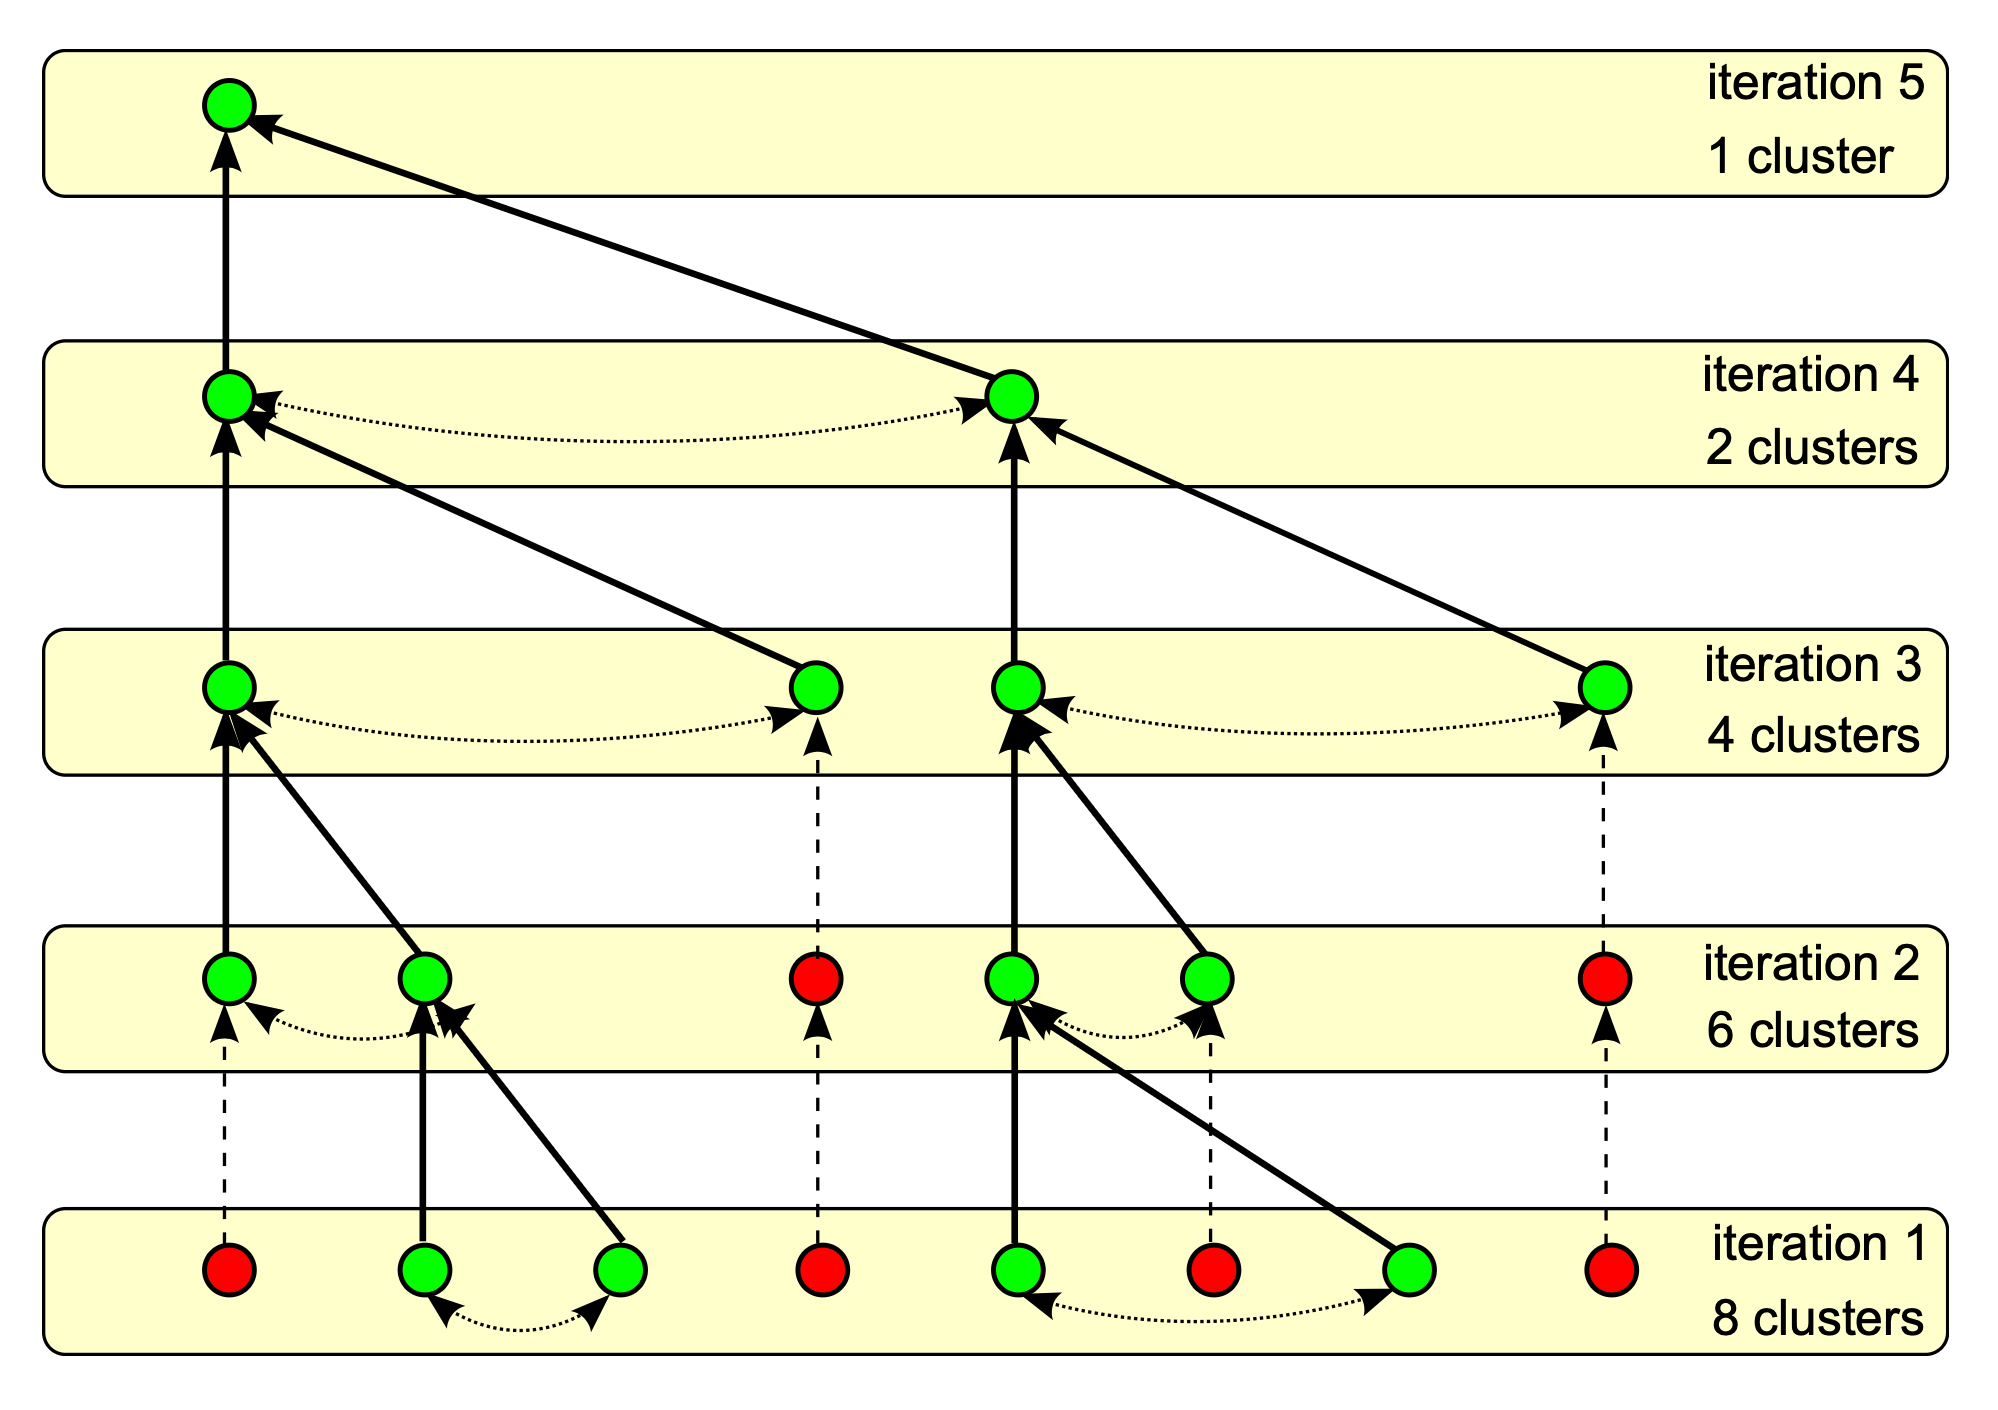
\includegraphics[width=0.8\linewidth]{images/PlocIterations.png}
    \caption{PLOC iterations. In each iteration, mutually corresponding clusters are merged (green nodes connected by dots). Newly merged clusters (green nodes deriving from two nodes from the previous iteration) and untouched clusters (red nodes) enter the next iteration. \cite{MB17}}
    \label{fig:ploc-iterations}
\end{figure}

\definecolor{nncolor}{RGB}{180,0,0}
\definecolor{mergecolor}{RGB}{0,180,0}
\definecolor{compactcolor}{RGB}{0,0,180}

Clusters are stored in two buffers (input and output), along with additional buffers to store the nodes of the resulting BVH, triangle indices, and several temporary buffers.

The algorithm starts by precomputing the bounding boxes and the Morton codes of scene primitives. It then sorts the primitives to order them along the Morton curve. Initially, all clusters are of size one, with one triangle in each.

The main loop starts and runs through a number of iterations. In each iteration, all nearest neighbor cluster pairs are merged. The main loop is made up of three phases: nearest neighbor search, merging, and compaction. After finishing each iteration, the input and output buffers are swapped. This repeats until there is only one cluster left. To guarantee that the main loop finishes and to solve the rare case of completely equidistant clusters, the algorithm prioritizes the nearest neighbor with the lower index. A depiction of several iterations of the algorithm can be seen in Figure \ref{fig:ploc-iterations}. \cite{MB17}

The pseudocode is shown in Algorithm \ref{alg:ploc}. The highlighted three main phases of the algorithm are:

\begin{itemize}
    \item The \textit{nearest neighbor search} phase (shown in {\color{nncolor} red}) searches for each cluster's nearest neighbor along the Morton curve in parallel using the 1D interval of clusters in the input buffer. Parameter $r$ denotes the interval, and it is clipped to prevent \textit{out-of-bounds} memory access. Each cluster keeps the nearest neighbor found (based on distance function $d$).
    \item The \textit{merging} phase (shown in {\color{mergecolor} green}) checks if each cluster is equal to its nearest neighbors nearest neighbor in parallel. If that is true, then both clusters are merged into one. To avoid conflict, the cluster with the lower index performs the merge. The first cluster (lower index) is replaced with the newly merged cluster, and the second cluster (higher index) is marked as invalid. At the same time, the algorithm creates a corresponding interior node for the new cluster. To determine the indices of the new interior nodes, a parallel prefix scan is performed on the new clusters. By adding the prefix scan value to the node counter, we can determine the actual node indices.
    \item The \textit{compaction} phase (shown in {\color{compactcolor} blue}) performs an exclusive parallel prefix scan to remove invalid clusters. The position of the node indices is determined by the prefix scan values and written to the output buffer. After some of the clusters have been merged and gaps appear in the Moron curve, a global prefix scan is needed to remove them. Note that the new clusters are not sorted again according to the Morton codes of their centroids. The authors observed that the clusters keep their ordering, which is sufficient enough for the nearest neighbor search algorithm, and so costly sorting can be avoided.
\end{itemize} 

\begin{algorithm}[h!tb]
\caption{PLOC algorithm pseudocode. The input of the algorithm is a sequence of $n$ clusters $C_0, C_1, \dots , C_{n-1}$ sorted along the Morton curve. Two auxiliary arrays are used: $\mathcal{N}$ (nearest neighbor indices) and $\mathcal{P}$ (exclusive prefix scan). The symbol $\emptyset$ denotes an invalid cluster. \cite{MB17}}
\label{alg:ploc}
\begin{algorithmic}[1]
    
\State $\mathcal{C}_{in} \gets \mathcal{C}_{out} \gets [C_0,\dots,C_{n-1}]$
\State $\mathcal{N} \gets \mathcal{P} \gets [0,\dots,n-1]$
\State $c \gets n$

\While{$c>1$}
    \For{$i \gets 0$ to $c-1$ \textbf{in parallel}}
        
        \color{nncolor}
        \State /* \textsc{Nearest Neighbor Search} */
        \State $d_{\min} \gets \infty$
        \For{$j \gets \max(i-r,0)$ to $\min(i+r,c-1)$}
            \If{$i \ne j \land d_{\min} > d(\mathcal{C}_{in}[i],\mathcal{C}_{in}[j])$}
                \State $d_{\min} \gets d(\mathcal{C}_{in}[i],\mathcal{C}_{in}[j])$
                \State $\mathcal{N}[i] \gets j$
            \EndIf
        \EndFor
        
        \color{black}
        \State $\textsc{Barrier}()$
        
        \color{mergecolor}
        \State /* \textsc{Merging} */
        \If{$\mathcal{N}[\mathcal{N}[i]] = i \land i < \mathcal{N}[i]$}
            \State $\mathcal{C}_{in}[i] \gets \textsc{Cluster}(\mathcal{C}_{in}[i],\mathcal{C}_{in}[\mathcal{N}[i]])$
            \State $\mathcal{C}_{in}[\mathcal{N}[i]] \gets %\color{black}\emptyset\color{compactcolor}$
            \emptyset$
        \EndIf
        
        \color{black}
        \State $\textsc{Barrier}()$
        
        \color{compactcolor}
        \State /* \textsc{Compaction} */
        \State $\mathcal{P}[i] \gets \textsc{PrefixScan}(\mathcal{C}_{in}[i] \ne %\color{black}\emptyset\color{compactcolor}$
        \emptyset)$
        %\If{$\mathcal{C}_{in}[i] \ne \color{black}\emptyset\color{compactcolor}$}
        \If{$\mathcal{C}_{in}[i] \ne \emptyset$}
            \State $\mathcal{C}_{out}[\mathcal{P}[i]] \gets \mathcal{C}_{in}[i]$
        \EndIf
        
        \color{black}
        \State $\textsc{Barrier}()$
        
    \EndFor
    
    \State $c \gets \mathcal{P}[c-1]$
    
    \If{$\mathcal{C}_{in}[c-1] \ne \emptyset$}
        \State $c \gets c+1$
    \EndIf
    
    \State $\textsc{Swap}(\mathcal{C}_{in},\mathcal{C}_{out})$
    
\EndWhile

\end{algorithmic}
\end{algorithm}


% ----------------------------------------
\clearpage
\section{Extended Morton codes for BVH construction}

Extended Morton codes \cite{Vinkler2017} propose to extend Morton codes, which are used for spatial sorting of scene primitives. These extensions increase the clustering and coherence from object sorting. They improve the primitive sorting especially well in non-uniformly distributed scenes. The proposed extensions enhance the basic Morton code by encoding object size, applying adaptive ordering of the individual bits, and using variable bit counts for different axes. Extended Morton codes lead to higher quality BVH, particularly for BVH build algorithms that heavily rely on spatial coherence of Morton code sorting. The method is easy to implement into algorithms that already use Morton codes and does not increase the build time significantly.

\subsection{Morton code based spatial sorting}

\subsubsection{Morton codes}

Morton code is a space filling curve that provides relatively coherent ordering of quantized vectors, meaning that continuous Morton code sequences are spatially close together. Morton code maps quantized n-dimensional vectors into integer scalar values - codes. The resulting curve of consecutive codes is also known as the Z-curve because of its shape when used with 2D data (see Figure \ref{fig:morton-space-filling}). Many more space filling curves exist and some with even more coherent spatial ordering \cite{Samet2006}, but Morton code became popular due to its simplicity and cheap computation time using only bit interleaving operations.

The Morton code is made up of a set number of bits that serves as its major parameter, along with the number of dimensions. An \(n\) bit Morton code of a three dimensional vector $v = (v_x, v_y, v_z) \in \langle 0, 1 \rangle^3$ is computed by first quantizing the coordinates $v^* = \{ v^*_x, v^*_y, v^*_z \} \in \langle 0,2^{n/3} \rangle \times \langle 0,2^{n/3} \rangle \times \langle 0,2^{n/3} \rangle$ and then the code is then constructed by interleaving bits of the components of $v^*$ \cite{Vinkler2017}. 

The bit interleaving operation can be performed using multiplication and sums as first conceived \cite{Morton1966}. Alternatively, precomputed lookup tables can be used for certain bit ranges and then combined by additions and shifts.

\begin{figure}[h!tb]
\centering
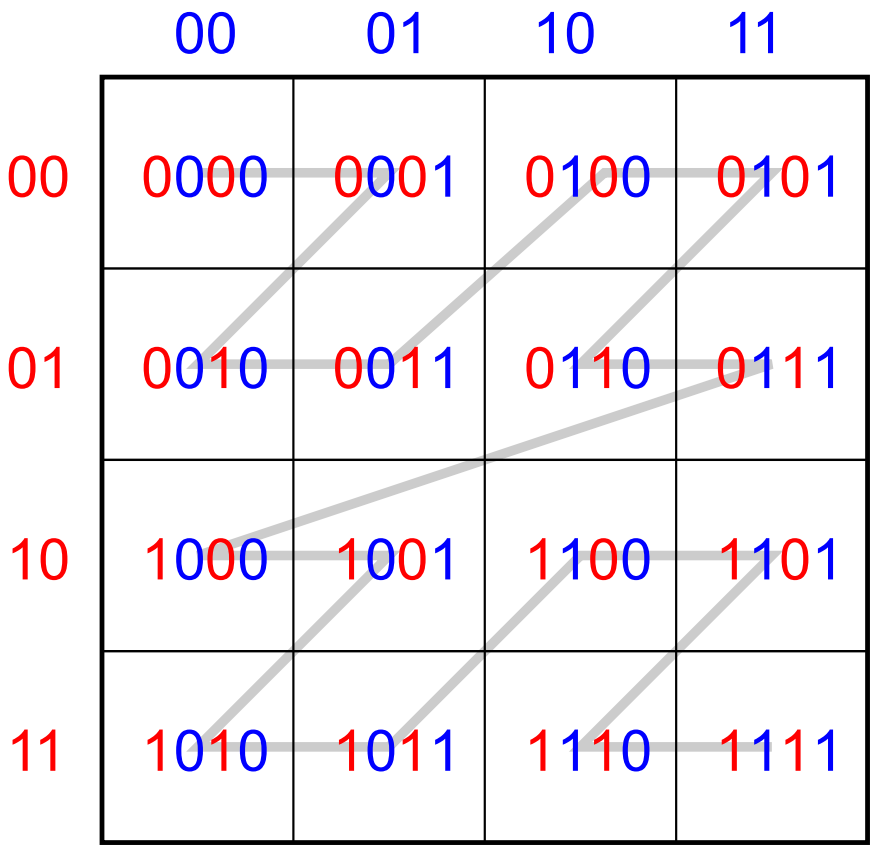
\includegraphics[width=0.8\textwidth]{images/MortonCodeSpaceFilling.png}
\caption{Space-filling curve representation of Morton codes in 2D space 
\cite{Vinkler2017}.}
\label{fig:morton-space-filling}
\end{figure}

\subsubsection{Constructing BVH using Morton codes}

Since Morton codes encode the spatial location of positions in 3D space, they can be easily used for the construction of spatial data structures. Scene primitives are represented as points and sorted according to their individual Morton codes, by doing this multi-scale clusters of primitives can form. Boundaries between clusters are defined by changes in bit positions. \cite{Vinkler2017}

This property is exploited by spatial data structures that use Morton codes. For example, the LBVH method \cite{Lauterbach2009} sorts primitives according to the Morton codes of their centroids. Starting from the most significant bit, the BVH tree is formed by splitting the current node (starting from the root with all primitives) in two according to the value of the bit in the centroid of the primitive at that position. Thus, the BVH topology is solely given by the computed Morton codes.

\subsection{Extended Morton codes}

This section summarizes the individual extensions proposed to the standard Morton Codes. These extensions modify the encoded data, their ordering, and the number of bits dedicated to each axis (or other encoded data).

\subsubsection{Encoding object size}

Real-world scenes typically contain geometric primitives with widely varying sizes. When primitives are sorted only by their centroid positions, spatial clustering can become inefficient. Although centroids may be spatially close, the resulting common bounding volume may be poorly fitted, particularly affecting smaller objects in the cluster. Large primitives propagate their larger bounding volumes not just at individual leaf nodes, but along the entire path from leaf to root, degrading overall BVH quality. Therefore, it is better to isolate such large objects and potentially position them at higher tree levels to minimize their influence on the remaining hierarchy. \cite{Vinkler2017}

The authors propose encoding the primitive size directly into the Morton code by injecting additional bits representing the diagonal length of the object. In the simplest configuration, the size information uses the same bit allocation as the three spatial axes, resulting in a 4-dimensional Morton code constructed by interleaving quantized coordinates $(x, y, z, s)$, where $s$ represents the primitive size normalized to the scene bounding box diagonal. With regular bit interleaving pattern (e.g., $xyzsxyzs...$), the resulting code structure mirrors octree-like subdivision, where each triple of spatial splits subdivides volumes into eight equal sub-volumes with half the original diagonal size. The size bits can then directly determine whether an object is larger or smaller than the current volume primitives. If the size bit is set to 1, the bounding box exceeds the dimensions of the current box and is separated into a distinct subtree, as can be seen in Figure~\ref{fig:morton-construction}. The authors also experimented with encoding the surface area instead of the diagonal length, but the diagonal length produced slightly better overall performance in their evaluation \cite{Vinkler2017}.

\begin{figure}[h!tb]
\centering
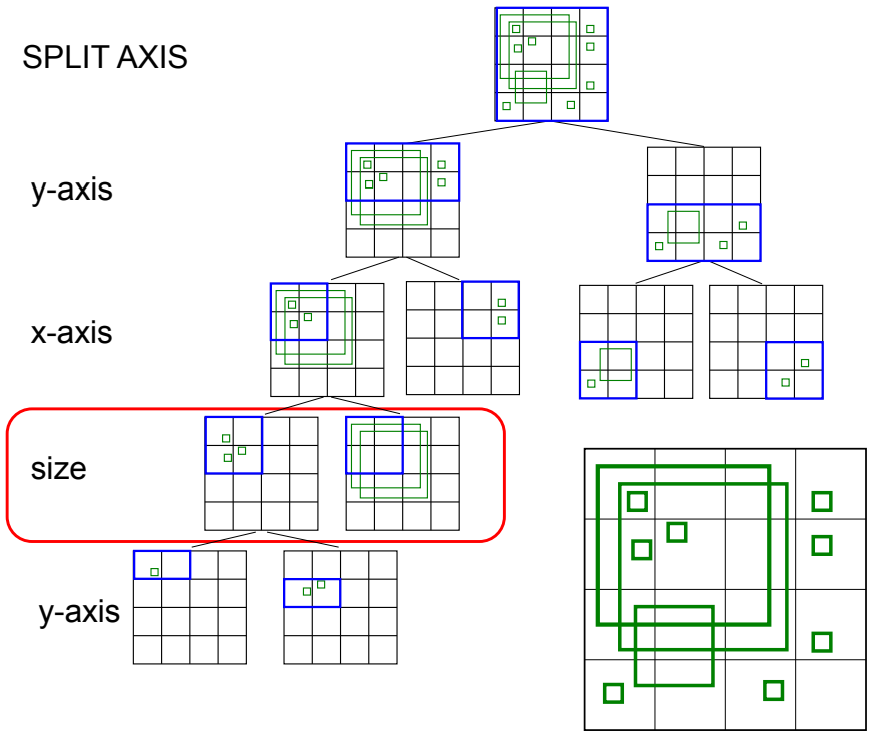
\includegraphics[width=0.8\textwidth]{images/MortonCodeConstruction.png}
\caption{Visual representation of Morton code construction in 3D space 
\cite{Vinkler2017}. Size bit is used to subdivide objects in the third level.}
\label{fig:morton-construction}
\end{figure}

\paragraph{Using fewer size bits} is beneficial in certain scenarios, particularly with shorter bit codes (32-bit Morton codes) or large scenes with many millions of primitives. Encoding object size in a coarser manner can be enough to preserve the primary subdivision potential of spatial positions. The authors propose reducing size bit allocation by injecting size bits only every 7th bit position - after two complete cycles of splits along each spatial axis - while maintaining the ability to separate small and large objects at appropriate tree levels. \cite{Vinkler2017}

\subsubsection{Adaptive axis order}

The authors discovered through experimentation that the ordering of spatial axis bits within the Morton code significantly influences BVH quality. Specifically, arranging axes in descending order by scene extent - placing the largest dimension first - consistently improved results, as splitting along larger axes first produces centroid clusters that are more cuboid-shaped and spatially compact compared to fixed $(xyz)$ ordering. \cite{Vinkler2017}

\subsubsection{Variable bit count}

The adaptive axis ordering concept can be generalized further by allowing variable bit allocation across different axes, which is particularly beneficial for scenes with non-uniform extents in individual axes, such as terrain or city models that extend primarily along two dimensions. The authors propose a major-axis-based method, where the largest axis is selected for each bit position, and the bounding box is halved along that axis before the next bit selection. Injection of optional size bits is made at regular intervals (every 4th or 7th bit). Once all bits are assigned, the bit counts per-axis determine the appropriate quantization scales. \cite{Vinkler2017}

\subsubsection{Extension combinations}

Two versions are suggested by the original article. The pseudocode for version~1: the 64-bit EMC generation using adaptive axis order and size bits injected every 4th bit can be seen in Algorithm~\ref{alg:emc64var1}.The pseudocode for version~2: the 64-bit EMC generation using variable bit order, adaptive axis order, and size bits injected every 7th bit can be seen in Algorithm~\ref{alg:emc64var2}. The \textsc{Expand} function inserts a variable number of zeroes before each bit of the input number. Notation: $X \ll Y$ corresponds to the left shift bitwise operation of integer $X$ by $Y$ bits, $\mid$ corresponds to the bitwise binary operation OR, and $\&$ corresponds to the bitwise binary operation AND. \cite{Vinkler2017}

% EMC Variant 1
\begin{algorithm}[H]
\caption{Pseudocode of the 64-bit EMC variant 2 generation. \cite{Vinkler2017}}
\label{alg:emc64var1}
\begin{algorithmic}[1]

\Function{Init}{$scene$}
  \State $a_0 = x,\; a_1 = y,\; a_2 = z,\; a_3 = size$
  \State \Call{sort}{$a_0..a_2$} \Comment{descending axis order using scene dimensions}
  \Comment{compute quantization scales}
  \State $s_0 = 2^{16} / scene.box.size[a_0]$
  \State $s_1 = 2^{16} / scene.box.size[a_1]$
  \State $s_2 = 2^{16} / scene.box.size[a_2]$
  \State $s_3 = 2^{16} / scene.diagonal.length$
\EndFunction

\Function{Expand}{$X$}
  \State $v = 0,\; mask = 1$
  \For{$i = 0$ to $15$ step $1$}
    \State $v = v \mid ((X \& mask) \ll (3 \cdot  i))$
    \State $mask = mask \ll 1$
  \EndFor
  \State \Return $v$
\EndFunction

\Function{Code}{$triangle$}
  \State $v = triangle.box.center-scene.box.min$
  \State $size = triangle.box.diagonal.length$
  \State $v^*_0 = s_0 \cdot v[a_0]$
  \State $v^*_1 = s_1 \cdot v[a_1]$
  \State $v^*_2 = s_2 \cdot v[a_2]$
  \State $v^*_3 = s_3 \cdot size$
  \State \Return 
    $(\Call{Expand}{v^*_0} \ll~3) \;\mid\; 
      (\Call{Expand}{v^*_1} \ll 2) \;\mid\; 
      (\Call{Expand}{v^*_2} \ll 1) \;\mid\; 
      \Call{Expand}{v^*_3}$
\EndFunction

\end{algorithmic}
\end{algorithm}


\begin{algorithm}[h!tb]
\caption{Pseudocode of the 64-bit EMC variant 2 generation. \cite{Vinkler2017}}
\label{alg:emc64var2}
\begin{algorithmic}[1]

\Function{Init}{$scene$}
  \For{$i = 0$ to $63$}
    \If{$i$ is the 7th bit}
      \State $axes[i] = 3$ \Comment{insert size bit}
    \Else
      \State $axes[i] = scene.box.size.maxAxis$ \Comment{pick the largest axis}
      \State $scene.box.size.maxAxis /= 2$ \Comment{halve the largest axis}
    \EndIf
  \EndFor
  \State $bits_{0..3} = axes.sum(0..3)$ \Comment{number of bits in each axis}
  \State $shifts_{0..3} = axes.shifts(0..3)$ \Comment{shifts between bits in each axis}
  \Comment{compute quantization scales}
  \State $s_0 = 2^{bits_0} / scene.box.size[a_0]$
  \State $s_1 = 2^{bits_1} / scene.box.size[a_1]$
  \State $s_2 = 2^{bits_2} / scene.box.size[a_2]$
  \State $s_3 = 2^{bits_3} / scene.box.diagonal.length$
\EndFunction

\Function{Expand}{$axis,\; X$}
  \State $v = 0,\; mask = 1$
  \For{$i = 0$ to $bits_{axis}-1$}
    \State $v = v \mid ((X\ \&\ mask) \ll (shifts_{axis}[i]))$
    \State $mask = mask \ll 1$
  \EndFor
  \State \Return $v$
\EndFunction

\Function{Code}{$triangle$}
  \State $v = triangle.box.center - scene.box.min$
  \State $size = triangle.box.diagonal.length$
  \State $v^*_0 = s_0 \cdot v[a_0]$
  \State $v^*_1 = s_1 \cdot v[a_1]$
  \State $v^*_2 = s_2 \cdot v[a_2]$
  \State $v^*_3 = s_3 \cdot size$
  \State \Return
    $(\Call{Expand}{a_0, v^*_0}  \ll 3) \;\mid\;
      (\Call{Expand}{a_1, v^*_1} \ll 2) \;\mid\;
      (\Call{Expand}{a_2, v^*_2} \ll 1) \;\mid\;
      \Call{Expand}{a_3, v^*_3}$
\EndFunction
  
\end{algorithmic}
\end{algorithm}


% ----------------------------------------
\clearpage
\section{Skewed oriented bounding boxes}
\label{sec:sobb}

In the context of ray tracing, vast majority of BVH axis aligned bounding boxes (AABB) are used as the bounding primitives. Recently, tighter bounding volumes such as oriented bounding boxes (OBB) \cite{OR85} or discrete orientation polytopes (DOP) \cite{KZ97} have been discovered to improve the performance of ray tracing at the cost of increasing the BVH constriction time \cite{KB24}.

In the this section of the thesis, the Skewed oriented bounding boxes (SOBB) \cite{KB25} are introduced as a generalization of the oriented bounding box with the skew transformation. The resulting bounding primitive corresponds to a parallelepiped defined by three slabs. In the following sections, you can read about the geometry, surface area calculations, ray intersection, and BVH application of the SOBB.

\subsection{Definition of SOBB}

This section explains the SOBB as a shape. Firstly its geometric definition and then how to compute its surface area -- an essential operation for tightly fitting the primitives and clusters of primitives during BVH construction.

\subsubsection{Geometry of SOBB}

Skewed oriented bounding box is a bounding volume for a set of scene primitives, its geometrical representation corresponds to a \textit{parallelepiped}. A parallelepiped is an object comprised of three pairs of parallel faces, each being a parallelogram. Well known 3D objects, such as a cube or a rectangular cuboid, are general parallelepipeds with a set of edge and angle constraints. Cuboid shapes are especially important as bounding volumes for entities in computer graphics, either as AABBs or OBBs. \cite{KB25}

Multiple representations can be used to describe a parallelepiped: (1) The \textit{edge-based representation} consists of three edge vectors. These vectors are a basis for a vector space with parallelepiped edges with unit lengths aligned with the axes. (2) The \textit{slab-based representation} forms the parallelepiped as an intersection of three slabs, each comprised of two parallel planes defined by a normal vector and distances from origin. Both representations are illustrated in Figure \ref{fig:sobb-geometry}. For different computational tasks, one representation may be more beneficial than the other. \cite{KB25}

It is beneficial to maintain a single representation throughout the entire pipeline for efficiency. Slab representation is often favored because of the efficient ray-object intersection. \cite{KB25}

\begin{figure}[h!tb]
    \centering
    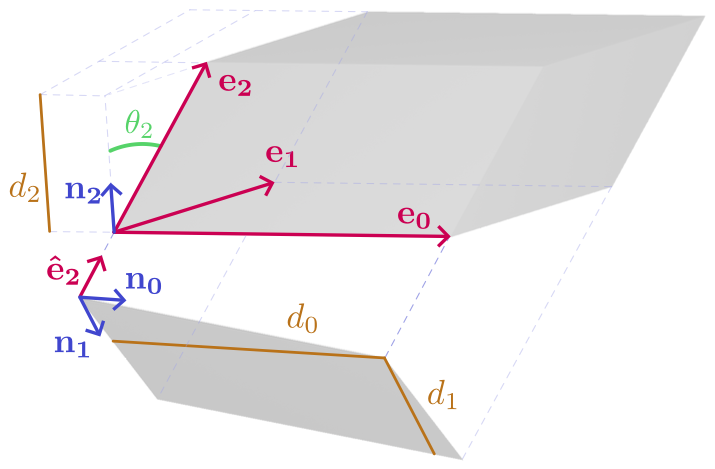
\includegraphics[width=0.8\linewidth]{images/SOBB_geometry.png}
    \caption{Parallelepiped with edges $e_0$, $e_1$ and $e_2$. Slab representation with slab normals $n_0$, $n_1$ and $n_2$ combined with their respective widths $d_0$, $d_1$ and $d_2$ \cite{KB25}.}
    \label{fig:sobb-geometry}
\end{figure}

\subsubsection{Surface area of SOBB}

Surface area is on the other hand (unlike ray-object intersection) more easily formulated in the edge representation. The surface area formula for a parallelepiped with edges $e_0$, $e_1$ and $e_2$ (as shown in Figure \ref{fig:sobb-geometry}) is formed by summing the area of the face parallelograms \cite{KB25}:
\begin{align}
    A_{pp}(\mathbf{e}_0, \mathbf{e}_1, \mathbf{e}_2)
        &= 2 \big( A_{pg}^0(\mathbf{e}_0, \mathbf{e}_1)
        + A_{pg}^1(\mathbf{e}_1, \mathbf{e}_2)
        + A_{pg}^2(\mathbf{e}_2, \mathbf{e}_0) \big) \notag \\
        &= 2 \big( \lvert \mathbf{e}_0 \times \mathbf{e}_1 \rvert
        + \lvert \mathbf{e}_1 \times \mathbf{e}_2 \rvert
        + \lvert \mathbf{e}_2 \times \mathbf{e}_0 \rvert \big)
    \label{eq:sobb-edge-surface-area}
\end{align}

To compute each parallelogram's surface area, the following formula can be used \cite{KB25}:
\begin{equation}
    A_{Pg}^{0}(\mathbf{e}_{0}, \mathbf{e}_{1}) = \lvert \mathbf{e}_{0} \times \mathbf{e}_{1} \rvert = \lvert \mathbf{e}_{0} \rvert \lvert \mathbf{e}_{1} \rvert \sin \alpha_{0} = \lvert \mathbf{e}_{0} \rvert \lvert \mathbf{e}_{1} \rvert \lvert \hat{\mathbf{e}}_{0} \times \hat{\mathbf{e}}_{1} \rvert
    \label{eq:pg-edge-surface-area}
\end{equation}
or transformed to the slab notation and simplified using the scalar triple product\cite{KB25}:
\begin{equation}
    A_{pg}^{0}(\mathbf{n}_{0}, \mathbf{n}_{1}, \mathbf{n}_{2}, d_{0}, d_{1}) = \ldots = \frac{d_{0} d_{1}}{\left| \det \big[ \mathbf{n}_{0} \ \mathbf{n}_{1} \ \mathbf{n}_{2} \big] \right|}
    \label{eq:pg-slab-surface-area}
\end{equation}

Surface area computation is especially important for BVH construction, so to avoid transitioning between slab and edge representations, the authors derived a formula for surface area computation for the slab representation \cite{KB25}:
\begin{equation}
    A_{pp}(n_0, n_1, n_2, d_0, d_1, d_2)
    = 2 \left( \frac{d_0 d_1 + d_1 d_2 + d_2 d_0}{\left|\det\left[\,n_0 \quad n_1 \quad n_2\,\right]\right|} \right)
    \label{eq:sobb-slab-surface-area}
\end{equation}

Equation \ref{eq:sobb-slab-surface-area} indicates that the surface area of a parallelepiped is inversely related to both the absolute value of the determinant of the matrix formed from the normal vectors of the slab and the volume of the unit parallelepiped generated by the normals of the slabs that determine the original parallelepiped. This volume (the value of the determinant) can serve as an indicator of orthogonality of the basis of the parallelepiped. \cite{KB25}

\subsection{Construction and traversal of SOBB BVH}

This section reveals the algorithm for building SOBB and SOBB BVH. It also talks about the traversal of such BVH and about the associated memory consumption and layouts.

\subsubsection{SOBB construction using $k$-DOPs}

Each processed set of primitives is fitted with a high degree $k$-DOP, which is then sampled for a triplet of slabs. These three chosen slabs form the newly created SOBB and are stored in the final hierarchy. \cite{KB25}

As hinted earlier, a $k$-DOP consists of $k$ parallel planes defined by $k/2$ pairs of collinear but opposing normals. The candidate SOBB set is based on the discrete set of $k$-DOP normals, consisting of all combinations of three normals. Generally, a uniform distribution of normals should be aimed for. However, it may be practical to ensure that certain normal directions are available, such as those of an orthogonal AABB basis. The discrete sets of normals are obtained by the relaxation of random samples on the surface of a unit hemisphere. The size of the candidate set increases with the rate of $(k/2)^3$ (assuming that all normals are linearly independent). This has the effect that, even though higher $k$ values are likely to create better fitting SOBB, the space of candidates grows rapidly outside of computable feasibility. \cite{KB25}

The surface area of the SOBB is used to choose the best fitting SOBB. Candidate SOBBs are generated using the intermediate $k$-DOP representation and one of the following strategies:

\paragraph{$O(k^3)$ strategy.} Brute force can be used to find the optimal SOBB for the given $k$-DOP by iterating over all SOBBs generated by the $k$-DOP triples, evaluating Equation \ref{eq:sobb-slab-surface-area} for each triplet. Then the triplet with the smallest surface area is chosen. The construction performance is significantly affected by the three nested loops, but provides the best possible BVH for given $k$-DOP. \cite{KB25}

\paragraph{$O(k^2)$ strategy.} To speed up construction, it is possible to make a trade-off: A basis vector is preselected, and then all available normal pairs are evaluated for surface area using Equation \ref{eq:sobb-slab-surface-area}. Since the goal is to minimize the total area, the normal with the narrowest slab present in the $k$-DOP is selected as the first axis. \cite{KB25}

\paragraph{$O(k)$ strategy.} If the previous strategy is still too expensive (for high $k$ values) an even faster heuristic can be used. The three vectors are picked one by one, using the limited information for each step. The first axis is chosen in the same way as in the $O(k)^2$ strategy, by choosing the normal with the narrowest slab. The second axis is chosen in a way to minimize the area of the resulting parallelogram formed by the two normals. It can be computed with the inverted Equation \ref{eq:pg-edge-surface-area}, so while working in the slab representation: $A_{pg} = d_0d_1 / sin\theta$, with $d$ being the slab width and $\theta$ the angle between the tested normals. As the first normal has already been set at this time, the equation can be simplified to $A_{pg} = d^2 / (1 - (n_0 \cdot n_1)^2)$. The final surface area of the SOBB face will be scaled proportionally using the last axis of the basis, which is unknown at this point. To select the last vector and form the final SOBB, we again iterate through the available normals and choose the one that minimizes the surface area generated by the triplet. \cite{KB25}

\subsection{SOBB BVH construction}

The construction is based on an existing AABB hierarchy, which is transformed into an SOBB hierarchy in a single bottom-up pass. The correctness of the bottom-up pass is guaranteed by using atomic operations and the fact that all child nodes are always processed before their parent. \cite{KB25}

The main task is to transform the AABB bounding volume into an SOBB bounding volume for each node. 

The transformation algorithm works like this. For each leaf node, a $k$-DOP is fitted to the geometry stored in the node by projecting the geometry on the $k$-DOP normals. Then the space of possible SOBBs generated by the $k$-DOP fitting is explored, and the best candidate is chosen to create the final SOBB of the leaf. For internal nodes, the bottom-up traversal continues by applying almost the same process, except to construct the node's $k$-DOP the algorithm merges the children $k$-DOPs instead of fitting all included geometries. \cite{KB25}

\subsubsection{Memory layout and intersection test}

The SOBB representation right after construction comprises the triples normals, each associated with a minimal and maximal projection. This totals $15$ floating-point values, which can be stored in multiple ways. Each storage strategy directly impacts the intersection test performed during traversal. \cite{KB25}

\paragraph{Direct slab normals layout.} Each slab is represented as four floating-point values by scaling the normal and storing the factor \cite{KB25}:
\begin{equation}
    \rho = \frac{1}{\max(p_{\max} - p_{\min}, \epsilon)}, \quad
    \mathbf{s} = \rho \cdot \begin{bmatrix} n_x & n_y & n_z & p_{\min} \end{bmatrix}^{T}
    \label{eq:sobb-direct-slab-layout}
\end{equation}

The intersection test then uses the standard branchless slab-based ray clipping test, with decoded slab values using the computed scaling. The SOBB with its three basis vectors can be stored using $12$ floating-point values, $48$ bytes per volume (in single precision). \cite{KB25}

\paragraph{Transformation matrix layout.} A bijective linear transformation from one parallelepiped to another can be found (assuming non-degenerate volumes). From this transformation it is possible to find a linear transformation of the SOBB to a unifrom $[-0.5, 0.5]^3$ AABB. The representation then stores the inverse of the affine transformation matrix as a $3 \times 4$ matrix representation of the SOBB. During traversal the transformation matrix is utilized to transform the given ray and perform the intersection test in the space of the unit AABB \cite{SVCNM21}. Like the slab normals, one bounding volume requires $48$ bytes of memory (again in single precision). \cite{KB25}

\paragraph{Indirect slab normals layout.} This representation saves significantly on used memory by not storing the three normals per SOBB explicitly, but instead storing only an index into a shared buffer of precomputed normals. Each slab is then represented only by its minimum and maximum projection values together with the corresponding normal index.

The normal indices require only a small number of bits (depending on $k$), resulting in $24$ bytes for storing the single-precision slab spans, with an additional $2$ bytes used to store the three normal indices. For example, for ($k = 64$), each index requires $5$ bits, i.e., 15 bits in total, which can be compactly stored in 2 bytes.

During ray--SOBB intersection, the corresponding normals must be fetched from the shared buffer. After this indirection, the standard branchless slab-based ray clipping test can be used without any further modifications.

